\documentclass[9pt,a4paper]{article}
\usepackage[T1]{fontenc}
\usepackage{times}
\usepackage{tikz}
\usepackage{ictamxs}
\usepackage{graphicx}
\usepackage{caption}
\usepackage{amsmath}
\usepackage{multicol}
\usepackage{indentfirst}
\usepackage{geometry}
\usepackage{bm}

\captionsetup[figure]{labelsep=period, name={Figure}, font=small}
\captionsetup[table]{labelsep=period, name={Table}, font=small}

\setlength{\textheight}{250mm}
\setlength{\topmargin}{-21mm}
\setlength{\textwidth}{16.5cm}
\setlength{\oddsidemargin}{-1mm}

\def\thefootnote{}
\begin{document}

\title{Nearest particle microstucture in rising monodisperse suspensions of drops}
%
\authors{
\underline{Nicolas Fintzi}$^1 $, Jean-Lou Pierson$^1 $ \& St\'ephane Popinet$^2$$^{\rm *}$}
%
\footnotetext {\hskip -0.5cm\scriptsize $^{\rm *}$ Corresponding
author. E-mail: nicolas.fintzi@etu.sorbonne-universite.fr}

\affiliations{
$^1$IFP Energies Nouvelles, Rond-point de l'echangeur de Solaize, 69360 Solaize\\
$^2$CNRS \& Sorbonne Universit\'e, Institut Jean le Rond $\partial$'Alembert, 4 place Jussieu, 75252 PARIS CEDEX 05, France
}
%

\maketitle


\begin{summary}
    Buoyancy-driven droplet flows are encountered in many chemical engineering processes such as gravity separators, liquid-liquid extractors, etc. The usual engineering practice to model such facilities is to make use of the averaged Navier-Stokes equations and population balance equations. 
    However, these methods necessitate closure laws and a deep understanding of particle pair statistics.
    Therefore, within a multiscale strategy, we perform tri-periodic Direct Numerical Simulations (DNS) of monodisperse buoyancy driven suspension of drops.
    In addition to providing data for the closure terms appearing in averaged models, the simulations are of great interest to understand and describe the microstructure of suspensions. 
    In this work we present a concise analysis of the microstructure by analyzing the \textit{Nearest Particle Statistics} recently revisited by [3].  %the properties of pairs of particles, within the framework of 
\end{summary}

\section*{methodology}
\setlength{\parindent}{10pt}
\vspace*{-10pt}

To achieve tri-periodic simulations, we used a cubic multigrid mesh, implemented within the open-source Basilisk solver,
inside which we initialized an array of 125 droplets subjected to buoyancy forces only. 
The two-phase Navier--Stokes equations are discretized with a centered scheme and a geometric volume of fluid method with a Piecewise Linear Interface Calculation. The surface forces are computed assuming a constant surface tension coefficient, with a well-balanced, height-function formulation.
% It reads,
% \begin{equation}
%     \frac{\partial \rho \textbf{u}}{\partial t} +\bm{\nabla}\cdot(\rho \textbf{uu}) = \bm{\nabla} \cdot \bm{\sigma} + \rho \textbf{g} + \textbf{f}_\sigma \delta_S,
% \end{equation}
% \begin{equation}
%     \bm{\nabla} \cdot \textbf{u} = 0,
% \end{equation}
% where $\delta_S$ is the surface distribution function, $\textbf{f}_\sigma$ the surface force defined as the curvature times the surface tension coefficient along the normal of the droplet surface. 
% $\bm{\sigma} = -p \textbf{I} + \mu_f [\nabla \textbf{u}+ (\nabla \textbf{u})^T]$, with $p$ the pressure, is the Newtonian stress tensor and $\textbf{g}$ is the gravitational acceleration.
We introduce a novel algorithm designed to prevent the automatic numerical coalescence of droplet associated with the VOF representation.
This enables us to study a steady population of droplets within time, in our case a monodisperse distribution of droplets.
Besides, we change the simulation reference frame by applying a constant acceleration on the whole domain so that the bulk velocity of the simulation remain zero.
%In this way we can carry out stable DNS for arbitrary durations.
In practice, we ran our simulations for at least 300 droplet inertial time scales in order to obtain converged statistics.

\begin{table}[h!]
    \centering
    % 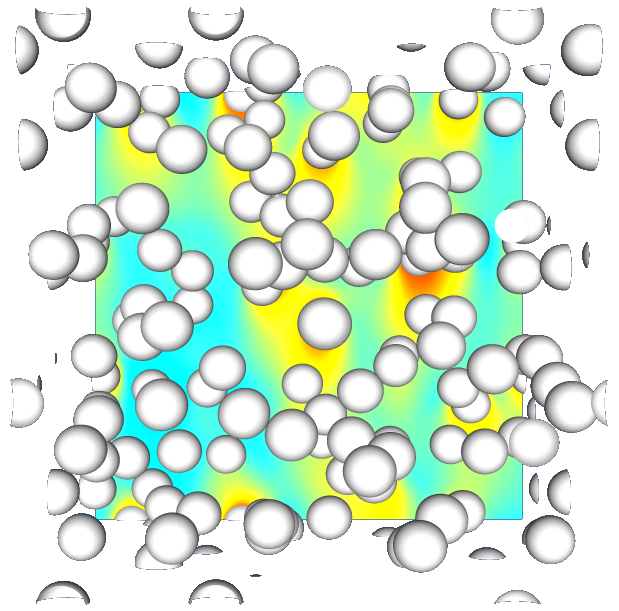
\includegraphics[width = 0.3\textwidth]{image/3D/P_PHI_5.png}

    \begin{tabular}{ccccccc}\hline
        $Ga$&$Bo$&$\phi$&$ \mu_r$&$\rho_r$\\ \hline\hline
        $[5;100]$&$[0.2;1]$&$[0.01;0.2]$&$[0.1;1]$&$1.111$\\ \hline
    \end{tabular}
    \vfill
    
    \caption{Dimensionless parameters investigated in this study.}
    \label{fig:pic}
\end{table}
The physical dimensionless parameters controlling this problem are the following. 
The \textit{Galileo number}, $Ga$, which is the ratio of the buoyancy forces over
the viscous forces.
The \textit{Bond number}, $Bo$, or the ratio between the buoyancy forces and surface tension forces.
The viscosity and density ratio are respectively noted, $\mu_r$ and $\rho_r$, (ratio of the dispersed phase over the continuous phase),
and the volume fraction of the dispersed phase is noted $\phi$. 
In this work we explored the range of parameters presented in Table \ref{fig:pic} (right) which correspond to the industrial applications mentioned in the summary.

\section{Results}
\setlength{\parindent}{10pt}
\vspace*{-10pt}

We present a statistical analysis of droplet interactions using the recent \textit{Nearest Particle Statistics} framework proposed by [3]. 
It consists in studying the interactions between the pairs of particles and their nearest neighbor only. 
By sampling particle-pair properties from the DNS presented above, it is possible to reconstruct any nearest pair probability density functions. 
Presently, we focus on the averaged relative positions of the particles that we describe with the nearest pair probability density function (PDF), $P_\text{nst}(\textbf{r})$.
This PDF represents the probability of finding the center of mass of a droplet at the position \textbf{r} knowing that its nearest neighbor's center of mass is located at $\textbf{r}=0$. 
We expect this PDF to depend on the dimensionless parameters, $Ga$, $Bo$, $\phi$, $\mu_r$ and $\rho_r$.
\begin{figure}
    \centering
    \begin{tikzpicture}
        \node (img1) at (0,1.7cm){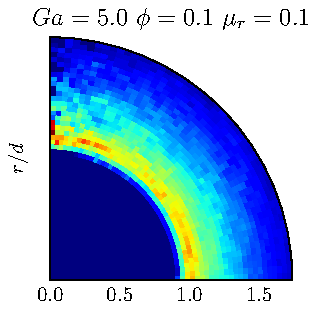
\includegraphics[width=3cm]{image/HOMOGENEOUS/fDrop/Pnst_mu_r_0_1_Ga_5_PHI_0_1}};
        \node (img2) at (3cm,1.7cm){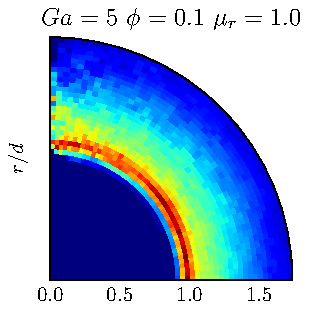
\includegraphics[width=3cm]{image/HOMOGENEOUS/fDrop/Pnst_mu_r_1_0_Ga_5_PHI_0_1}};
        \node (img3) at (0,-1.5cm){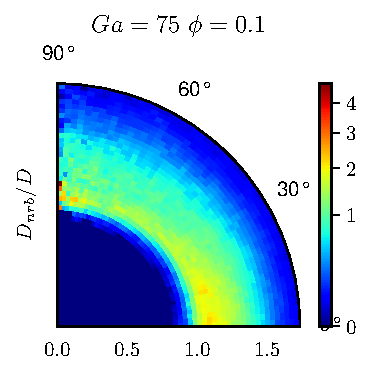
\includegraphics[width=3cm]{image/HOMOGENEOUS/fDrop/Pnst_mu_r_0_1_Ga_75_PHI_0_1}};
        \node (img4) at (3cm,-1.5cm){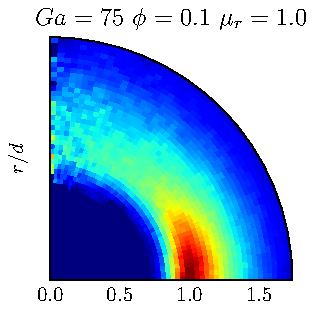
\includegraphics[width=3cm]{image/HOMOGENEOUS/fDrop/Pnst_mu_r_1_0_Ga_75_PHI_0_1}};
        \node (img5) at (7cm,0){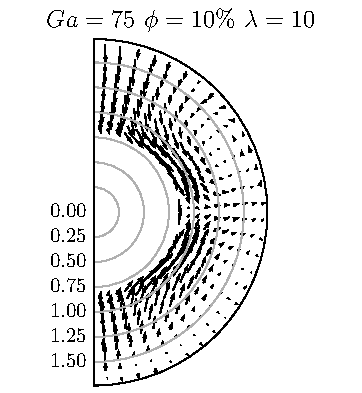
\includegraphics[width=5cm]{image/HOMOGENEOUS/fDrop/U_rel_l_10_Ga_75_PHI_10.pdf}};
        \node (img6) at (11.5cm,0){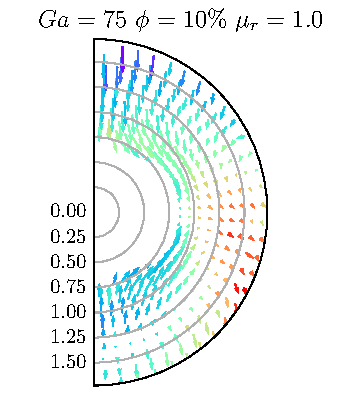
\includegraphics[width=5cm]{image/HOMOGENEOUS/fDrop/U_rel_l_1_Ga_75_PHI_10.pdf}};
        \draw (img1.south)node{(a)};
        \draw (img2.south)node{(b)};
        \draw (img3.south)node{(c)};
        \draw (img4.south)node{(d)};
        \draw (img5.south)node{(e)};
        \draw (img6.south)node{(f)};
    \end{tikzpicture}
    % \includegraphics[width=\textwidth]{tmp_img.png}
    \caption{[(a), (b), (c), (d)] Nearest particle probability density function $P_\text{nst}(\textbf{r})$ for two Galileo numbers ($5,75$) and two viscosity ratios ($0,1,1$).
    [(e), (f)] Averaged nearest particles relative velocity fields $\textbf{w}(\textbf{r},a)$ for respectively, $\mu_r = 0.1, 1$. The vector are coloured by the \textit{age of interaction} $a$. 
     }
    \label{fig:icmf}
\end{figure}
Figure \ref{fig:icmf} displays the probability density $P_\text{nst}(\textbf{r})$ reconstructed from a DNS with highly viscous droplets ($\mu_r=0.1$, solid-like droplets) and another one where the viscosity is the same for both phases ($\mu_r=1$ fluid droplets). The influence of inertia is also assessed using two \textit{Galileo} numbers: $Ga=5$ (low inertia) and $Ga=75$ (high inertia). 
It is seen that the pair distribution function for $Ga = 5$ (panel (a) and (b)) is isotropic while at higher $Ga$ (panel (c) and (d)) the distribution is larger on the horizontal sides. 
If we focus on the high-inertia cases (panel (c) and (d)), we can observe that the pair distribution function is slightly anisotropic for $\mu_r = 0.1$ and clearly anisotropic for $\mu_r = 1$ with a preferential probability of the nearest particle to be on the horizontal side. 
Additionally, a meticulous analysis of the radial probability density function $P_\text{nst}(|\textbf{r}|)$ (not shown here), leads us to the conclusions that particles are on average \textit{closer} with their nearest neighbor for $\mu_r =1$ and high $Ga$. 
This latter observation can be interpreted as the presence of more densely packed clusters for high inertia and moderate viscosity ratios (compared to low inertia and/or solid-like droplets) [4]. 

In a second step we present the averaged relative velocity fields $\textbf{w}(\textbf{r},a)$.
They represent the averaged relative velocity between a particle and its nearest neighbor, knowing that its nearest neighbor is located at the position $\textbf{r}$ with age $a$.
The \textit{age of interaction} $a$ is the time from which the neighboring particle became the nearest particle, to the current sample time. 
Figure \ref{fig:icmf} panel (e) and (f), display these velocity fields, the color map represents the value of the age, from dark blue for $a = 0$ to dark red for the longest interactions. 
Following the color map and the vector fields, it can be stated that on average, the nearest neighboring particles approach from the vertical directions and leave through the sides of the particle of reference. 
In fact, the fields $\textbf{w}(\textbf{r},a)$ provide a quantitative averaged representation of what is known as the \textit{Drafting Kissing Tumbling} [2] mechanism even if for $\lambda=1$ other non-viscous effects may be important [5].
%Indeed, the relative motions seem similar to those predicted by DKT.
Although not obvious on these plots, the velocity field for $\mu_r = 1$ exhibits a clear stagnation zone on the sides of the test particle.
Consequently the neighboring drops may end up on the lateral side of a given drop. %being pushed to the sides

% at the end of their interaction, which clearly explains the shape of $P_\text{nst}(\textbf{r})$ shown in Figure \ref{fig:icmf} panel (d). 
Regarding the case $\mu_r =0.1$, we observe slightly different kinematics, indeed the particles do not necessarily end their interactions on the sides, which partly explain the different form of $P_\text{nst}(\textbf{r})$ compared with the previous case.

\section{Discussion}
\vspace*{-10pt}
In this work, we carried out tri-periodic DNS of buoyancy driven motion of suspensions of drops for a wide range of dimensionless parameters. 
We provided evidence on the nature of the pairwise interactions by studying the probability density $P_\text{nst}(\textbf{r})$ and the relative conditional velocity field $\textbf{w}(\textbf{r},a)$. 
Within this framework  we could identify and quantify phenomena such as the DKT mechanism and the shape of the microstructure. 
% We demonstrate that $\mu_r$ and $Ga$ has a strong impact on the spatial arrangement of the particles and also on their relative behavior. 
% To fully understand to interaction mechanism in an emulsion, these arguments must be completed by a dynamical analysis of the interactions between particles, however, for succinctness it will not be presented in this document.  
This study has been motivated with the view of building a coalescence kernel for population balance equations. 
These coalescence models are often based on film drainage approximations which assume a normal approach between droplets [1].  
However, in Figure \ref{fig:icmf} (panel (e) and (f)), we showed that the interactions are more likely to happen tangentially rather than with a normal approach. 
We also demonstrated that $\mu_r$ and $Ga$ have a strong impact on the spatial arrangement of the particles and on their relative kinematics. 
For these reasons we conclude that there is a clear need to take in account these mechanisms, with the objective of building more accurate coalescence kernels. 
This could be done by considering more sophisticated film drainage situations which would consider relative velocities consistent with the $\textbf{w}(\textbf{r},a)$ distributions documented in this study.
This issue will be addressed in future work.  


\begin{thebibliography}{1}
    \bibitem{i}
    A. Chesters. Modelling of coalescence processes in fluid-liquid dispersions: a review of current understanding. Chemical
    engineering research and design, 69(A4):259–270, 1991.
    \bibitem{ii}
    A. F. Fortes, D. D. Joseph, and T. S. Lundgren. Nonlinear mechanics of fluidization of beds of spherical particles. Journal of
Fluid Mechanics, 177:467–483, 1987.
    
    \bibitem{iii}
    D. Z. Zhang. Ensemble average and nearest particle statistics in disperse multiphase flows. Journal of Fluid Mechanics, 910,
    2021.
    \bibitem{iv}
    D. Z. Zhang, M. Wang, and S. Balachandar. Evolution of the age-included nearest pair distribution in disperse multiphase
flows. Physics of Fluids, 35(6), 2023.
\bibitem{v}
D. Legendre, J. Magnaudet, and G. Mougin. Hydrodynamic interactions between two spherical bubbles rising
side by side in a viscous liquid. Journal of Fluid Mechanics, 497:133–166, 2003.
\end{thebibliography}
\end{document}
